\documentclass{article}

% PLOS One TEMPLATE
\usepackage{amsmath,amssymb,graphicx,cite,setspace}
\usepackage[textwidth=1.75in]{todonotes}
\usepackage[total={6in,9.5in},top=0.5in,left=0.5in,includefoot]{geometry}
\usepackage{listings}
\usepackage{url}
\usepackage{color}

% define Scala
\lstdefinelanguage{scala}{morekeywords={class,object,trait,extends,with,new,if,while,for,def,val,var,this},
otherkeywords={->,=>},
%procnamekeys={def,.},
sensitive=true,
keywordstyle=\color{magenta},
commentstyle=\color{green},
identifierstyle=\color{blue},
%procnamestyle=\color{black},
morecomment=[l]{//},
morecomment=[s]{/*}{*/},
morestring=[b]"}
% Default settings for code listings
\lstset{frame=tb,language=scala,aboveskip=3mm,belowskip=3mm,
showstringspaces=false,columns=flexible,basicstyle={\small\ttfamily}}
% handle tilde characters
\lstset{literate=%
{~}{\url{~}}1
}
% define no break code listing
\lstnewenvironment{code}[1][]%
{
   \noindent
   \minipage{\linewidth} 
   \vspace{0.5\baselineskip}
   \lstset{basicstyle=\ttfamily\footnotesize,frame=single,#1}}
{\endminipage}

\newenvironment{rnwfig}[0]{\begin{figure}\begin{center}}{\end{center}\end{figure}}

%\renewcommand{\lstlistingname}{Scala Code}

%\doublespacing

% Text layout
%\topmargin 0.0cm
%\oddsidemargin 0.5cm
%\evensidemargin 0.5cm
%\textwidth 16cm 
%\textheight 21cm

\usepackage[labelfont=bf,labelsep=period,justification=raggedright]{caption}

\newcommand{\Hub}[0]{\ensuremath{\mathbf{H}}}
\newcommand{\C}[1]{\ensuremath{\mathbf{C}_{#1}}}
\newcommand{\Obs}[0]{\ensuremath{\mathbf{O}}}
\newcommand{\todoCP}[1]{\todo{CP, #1}}

\usepackage{Sweave}
\begin{document}
\Sconcordance{concordance:manuscript.tex:manuscript.Rnw:%
1 70 1 1 0 632 1}

\begin{flushleft}
{\Large
\textbf{Modeling Requirements for Simulating Covert Social Groups}
}
% Insert Author names, affiliations and corresponding author email.
\\
Carl A. B. Pearson$^{1,\ast}$, 
Edo Airoldi$^{2}$,
Edward Kao$^{2}$,
Burton Singer$^{1}$, 
\\
\bf{1} Emerging Pathogens Institute, University of Florida, Gainesville, FL, USA
\\
\bf{2} Statistics, Harvard University, Cambridge, MA, USA
\\
$\ast$ E-mail: cap10@ufl.edu
\end{flushleft}
% Please keep the abstract between 250 and 300 words
\section*{Abstract}
Covert social groups are difficult to observe directly, by definition: members either actively thwart discovery or leverage passive features of their surrounding population to avoid detection.  Moreover, increasing active observation would be expected to perturb these social systems.  However, these groups never have perfect cover, their secrecy may make them conspicuously absent from the everyday activity of the background population, and finally there are potential mechanical charactericterizations -- their composition, goals, tactics, etc. -- that might predict their actions.

This situation -- strong constraints on passively and actively obtained direct empirical data, overwhelming indirect data, and competing mechanical explanations -- recommends simulation.  However, because the of the censoring issues in the data, that simulation requires particular attention to characterizing uncertainty and avoiding overfitting.

Herein, we discuss these issues in terms of network models.  Specifically, we review (i) incorporating observation uncertainty, (ii) the need for both back- and foreground populations, (iii) avoiding over-fitting, and (iv) finally some philosophy relative to implementation.

As part of that philosophical discussion, we walkthrough the exercise of procedurally generating back- and foreground populations, simulating communication among those individuals, and filtering those communications via an observation model.  We then address the issues of (i) fitting that model against data, and (ii) analyzing performance of the opposing sides (e.g. Receiver Operator Characteristic).  Finally, we also demonstrate a small extension.

%\todoCP{{\em I think not for this round, but maybe:} Finally, we consider the implications of {\em forged} messages.  In the basic model, we consider incomplete information about the communications, but the available information is always accurate.  In this extension, we allow the Observer and the clandestine group to forge messages.  We again measure various Observer performance traits relative to properties of the observed network.}

\newpage

\section*{Introduction}
For investigators ranging from anthropologists to law enforcement, the desire to find, study, and modify the behavior groups operating at the edge of the observable is a principle concern.  In the meta-theatre of the ironic, various media outlets have responded to public interest by applying this lens to the activities of intelligence organizations world-wide -- themselves desperate to undertake this very task against other clandestine actors.  Of course that revealation of these activities has broadly sparked the symmetric concern: being able to operate clandestinely in an age of ubiquitous monitoring.  Criminal organizations have long appreciated the value of operating in secret, as have groups subject to State-sponsored abuse or industrial espionage, and time will tell whether or not this spark catches fire in general behavior.

The underlying drive for these opposed efforts is the implacably expanding byte trail.  Once, the recorded information of an entire life might amount only to a few bytes -- parish records on births and deaths, perhaps including morbidity -- but now information era tools produce a near endless supply or 1s and 0s.  In some cases, this production is a side effect of organized commercial instinct -- monetizing search through targetted advertisement, e.g.  In other cases, individuals are voluntarily advancing their own brand -- Instagram ``selfies'', e.g.  However, in many cases this bitwise production is an engineering consequence of the associated technology.  E.g., cellular phones transmit constant location data, financial systems are increasingly just data-based, and of course any use of the internet produces veritable bit contrails.  This rate of production far exceeds the personal processing capability of any practically-sized team of analysts.

Hence, these teams employ computer-based, heuristic filtration to decide which data to record, to review, and to obtain.  We avoid saying ``algorithmic'' at this point: ``algorithmic'' implies strong, logically inevitable conclusions from inputs.  Like ``algorithmic'' bubble prediction, we tend to side more with Fama than Shiller.

Given the real uncertainty, what these filters call for is testing and validation, but those present their own difficulties.  Calling field testing ``problematic'' seems like a gross understatement; reference ``truth'' is either non-existent or deceptive, and experiments could have dangerous side effects.  Even making use of intensely studied historical events is problematic: these offer no way to consider evolutionary behavior and technological innovation (without even further abstraction), even assuming the historical data are more than victor's embellishment.

Generating synthetic data seems like an obvious alternative.  It allows for comparison across both detection and masking strategies, consideration of multiple background contexts, forecasting of risks and tradeoffs in a way that allows uncertainties, and in general providing a framework for imaginative assessment.  Like all such flexible tools producing quantitative results, it has the subtle downside of the simulator's biases being validated by numerical gospel; if one believes a particular strategy is effective -- perhaps even with reasonable agreement for a particular time and situation -- there would be a natural tendency to ``adjust'' scenarios until they indicated the success of strategy.

In the following sections, we lay out the uses and abuses of such a framework.  What makes for useful synthetic data sets?  What are the appropriate measures for detection strategies on them?  We motivate that discussion by inspiration from an over-simplified, network-based model of terrorism -- a sub-group of the Salafi jihad networks as described by Sageman {\em et al.}\cite{sageman} -- and community organization and communication.  Whether or not that work is an accurate description is not of particular concern.  Their qualitative properties are enough of a defensible testbed for modeling the communication patterns of one covert group.  We will point out where assumptions can be modified to identify different kinds of groups against a background population, since the behavior and structure of both the background and covert organizations are constantly evolving. 

\section*{Overview of the Simulation Problem}
Detecting a covert group is fundamentally about distinguishing the trace observable activity of that group from the activity of the background, bootstrapping that into guesses about the structure of the group, focusing the observation and distinguishing process based on that structure, and so on iteratively.  The purpose of simulation is ultimately to measure performance in the observer-covert group competition.

Given that these aspects must be expressed in the model (with varying degrees of detail), and that this model is used by a team or communicated between researchers, the language for that expression must be both powerful (to capture complexity where necessary), but also comprehensible to communicate what in fact is the meaning of the universe in this model.  Because these simulations are fundamentally about individuals and their behavior, we largely frame our discussion in terms of individuals, their internal state, and their interaction with others.

We can of course think in different terms.  For example, we are considering a network model of the population and covert group embedded within it, with edges representing relationships between people.  We might think of those relationships as being external state and correspondingly represent those relationships as external state in the simulation.  E.g., we might represent the population as a graph rather than a bag of individuals, and in the simulation the edges belong to the graph object rather than individuals.  As long as we recognize the translation between these perspectives, the choice boils down to what is most pragmatic relative to the science and simulation.  If most of the questions answered by the simulation relate to graph measures -- e.g., calculating various centrality measures -- then the simulation-as-graph rather than simulation-as-individuals probably makes more sense.

\subsection*{Modeling the Covert Groups}
Relative to the covert group, the simulation must model how the group members act and interact.  Typically, that further entails a modeling few moving pieces: (i) the members internal state (including what other members they know and communicate with), (ii) how that internal state evolves relative to external forces or states, and (iii) what actions those members undertake based on their internal state (possibly in response to some specific external event).

\subsection*{Modeling the Background}
Like the covert group, the background population is a (larger) group of individuals that act and interact.  They have the same basic modeling requirements as the covert group, but they behave differently.  This difference may be as simple as being distinct relative to observation process -- e.g., their communications are more likely to be recorded -- or it may be more noticeable like having fundamentally more diverse contacts, taking different kinds of actions, etc.

An alternative representation for the background would be to model it as a continuous entity vice individuals in a network.  This could be used to reduce the simulation size.  However, this model would still need to create activity data that was consistent (in format) to that created by the covert group.

\subsection*{Modeling Activity}
Individuals create modeled activity based on their internal state.  These actions correspond to (i) the observable events of specific interest (e.g., calls, financial transactions), (ii) generally observable events (e.g., travel, work, religious observations), and (iii) interactions that, while not externally observable, play a role in the evolution of internal state in other individuals either directly or by modifying the state of the world.  These actions should occur at specific times in the simulation, at whatever resolution is appropriate to the model.

The covert group and background population should be different in their activity; either performing different activities or undertaking them at different rates or on different schedules.

\subsection*{The Observation Model}

%To test strategies for either the covert group or survillience entity, one must have a model capable of representing their strategies.  That means modeling entities that take action, modeling how that action is observed (including if it is observed correctly, or at all), and modeling how those observations are digested into reactions.  Notably, the entities must include some sort of background -- if the only data being simulated is to do with the covert entities, they are hardly covert within that simulation.  Here, we will focus on network based models of these components.  Networks seem like a natural tool, given the role of individually-based action, discrete events, and the relatively small number of participants in these groups.  Though we do not do so in our example, the background population might be more tractably modeled with continuous phenomena, given its large size and potentially more homogeneous behavior.

%\subsection*{Modeling the Entities}
%For our motivating example, we divide the population into three types, two of which belong to the covert group -- management and subordinates -- and a third representing ordinary individuals in the background population.  We choose this number of types because we are using that many models of activity, though different degree nodes will present somewhat differently.  The background population may be less homogenous in types, or perhaps types may be better modeled as being selected from distribution of features.  What must be guarded against here is over fitting by mechanism -- essentially the problem of choosing a polynomial of power equal to the available data, but more subtle.  Fishing with different mechanics may yield a better historical fit, but not necessarily a better forecast.

%\subsubsection*{Background Population}
%Most observable action will be that of the general populace surrounding the clandestine group.  This population has some structural component -- {\em e.g.} family sizes, typical numbers of working members, tendency towards assortativity -- though not necessarily well-known when a given investigation begins and perhaps even assumed to be something it is not.  This structure is also likely dynamic due to natural evolution (or activity on the structure may change pattern dynamically, those perspectives not being easy to disentangle), or possibly in response to the investigation.  For example, the ongoing revelations about the NSA will no doubt influence the behavior of the technical elite and percolate into the general public.  Therefore, assessment of any particular pair of opposed strategies should cut across multiple models of the background, each independently parametrized around what data is available.

As an example background population, we have the ordinary individuals form small groups, which in turn connect into larger groups, those groups into still larger groups, and so on until the background consists of a single component.  If one were inclined to require that this description corresponded to a particular mechanism, this might loosely be interpreted as individuals forming households, households forming blocks, blocks forming neighborhoods, {\em ad nauseum}.  However, here it is only an academic fiction -- a compact, algorithmically and analytically convenient expression, without any connection to well-established mechanics or data.  If demographic data for households were available, then we could plausibly parameterize the lowest level, then possibly combine that with mortality and mobility data to characterize how closely connected households remained, and so on.

Independently, we establish a second set of edges with a different flavor.  The previously described edges we label ``Familial'', these we call ``Economic''.  We will generate these in an identical fashion.  Again, if one were inclined to propose an explanation, one might call these small businesses or groups within a business, those forming collaborating businesses or whole firms, and so on hierarchically.  Again, we emphasize: this choice is purely an academic fiction, where we have added this extra fiction purely to highlight the need for multiple dimensions to represent different kinds of relationships in the population.

For both of these types, the ``grouping'' operation is to try to form cliques of size $n$ (with allowance to handle an arbitrary total population size).  That is:\begin{enumerate}
\item create and randomly permute a population $P_0$, with $N$ members (later results use $N=100$).
\item\label{grouping_init} divide $P_0$ into equal groups of size $n$ (later results use $n=3$);
\item for each group $i$, completely connect the individuals, and label that group $C_i^0$
\item\label{grouping_end} form a population from the $C_i^0$
\item repeat steps \ref{grouping_init} to \ref{grouping_end} with the $C_i^0$ connecting each edge between the $C_i^0$ to a uniformly drawn individual within the group, then with the $C_i^1$, etc until a single component is obtained
\end{enumerate}

\begin{code}[title=Pseudo-Code: Hierarchical Cliques]
// form a clique from a vertex collection, col:
def clique(col : Collection[V]) =
    for ( (left, right) <- undirectedPairs(col) ) // for each unique, undirected pair in col:
      left <~> right // form a bidirectional edge across the pair
      
def hierarchicalClique(col: Collection[V], size:Int) = 
   val thisLvl : Collection[Collection[V]] =
     // make the lowest level cliques 
     for ( subGroup <- groupBySize(col, size) ) yield {
       clique(subGroup)
       subGroup
     }
   cliqueGroups(thisLvl, size)
   
  val thisLvl : Collection[Collection[V]] =
    // gather the groups being made into a higher level cliques
    for ( subGroups <- groupBySize(col, size) ) yield {
      // clique a group of groups
      for ( (leftGroup, rightGroup) <- undirectedPairs(subGroup) ) {
        leftGroup.randomMember <~> rightGroup.randomMember
      }
      // merge this set of subgroups into a single new group
      merge(subGroups)
    }
  // repeat with the cliqued cliques, unless everything has been connected
  if (thisLvl.size != 1) cliqueGroups(thisLvl, size)  
\end{code}

Lastly for this model, we establish a final set of edges with a third flavor: ``Religious''.  These edges occur between members with a probability based the distance between the individuals on the ``Familial'' graph.  That is -- for those wanting to assign a meaning -- members of the same family are most likely to observably interact in a religious capacity, then immediate relatives or neighbors, and so on.  Of course, this is again academic, chosen to illustrate that other generation algorithms are possible, even with dependence between dimensions.  The detailed algorithm is:\begin{enumerate}
\item\label{religious_init} for each individual $i$:
\item assign $d_i=1$ and $F_i$ to the set of all their familial connections, excluding individuals already considered
\item with probability $p^{d_i}$ connect $i$ to the members of $F_i$
\item\label{religious_end} increment $d_i$, move all of $F_i$ to $P_i$, then add all of the familial connections of $P_i$ that are not in $P_i$ (or previously considered) to $F_i$.
\item repeat steps \ref{religious_init} to \ref{religious_end} until $F_i$ has no members added in step \ref{religious_end} 
\end{enumerate}


\begin{rnwfig}
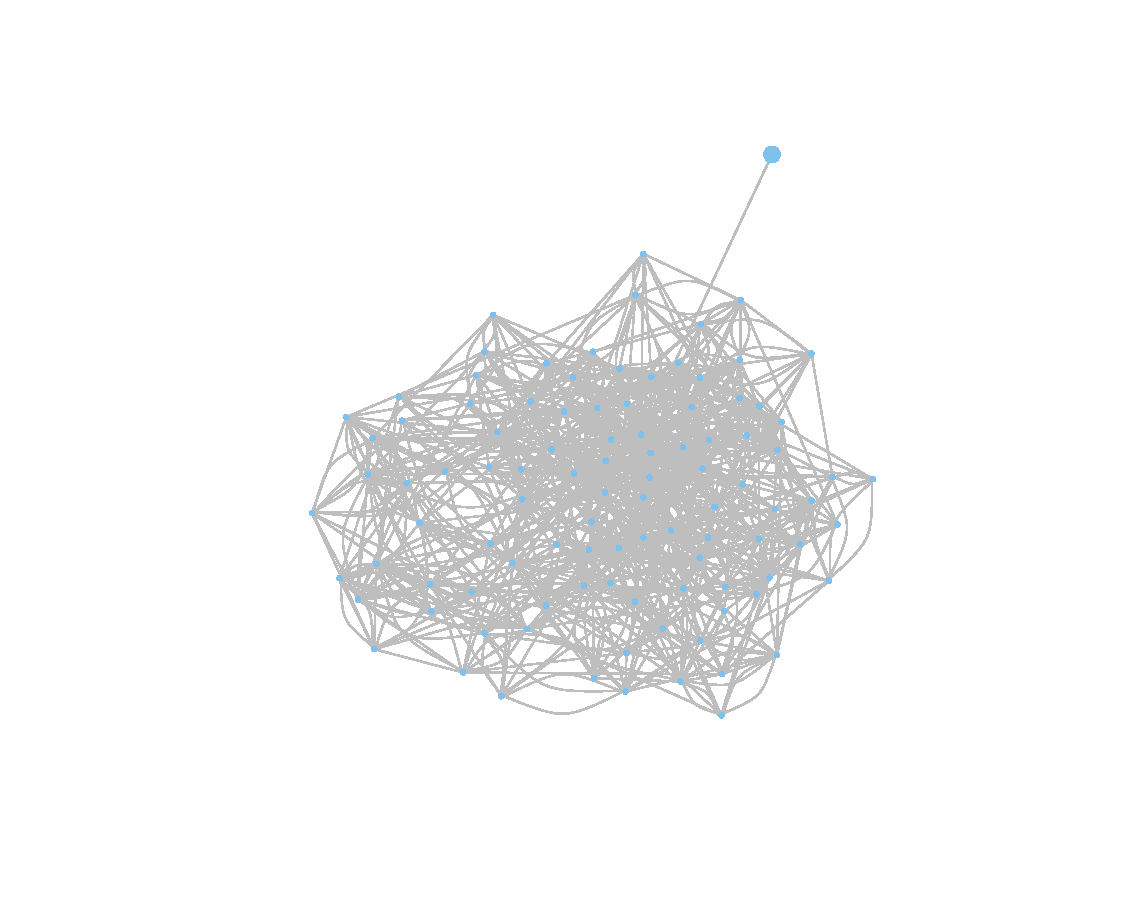
\includegraphics{manuscript-all}
\caption{Overlay of all connections; the large vertex represents the cluster of subordinates.}
\end{rnwfig}

\begin{rnwfig}
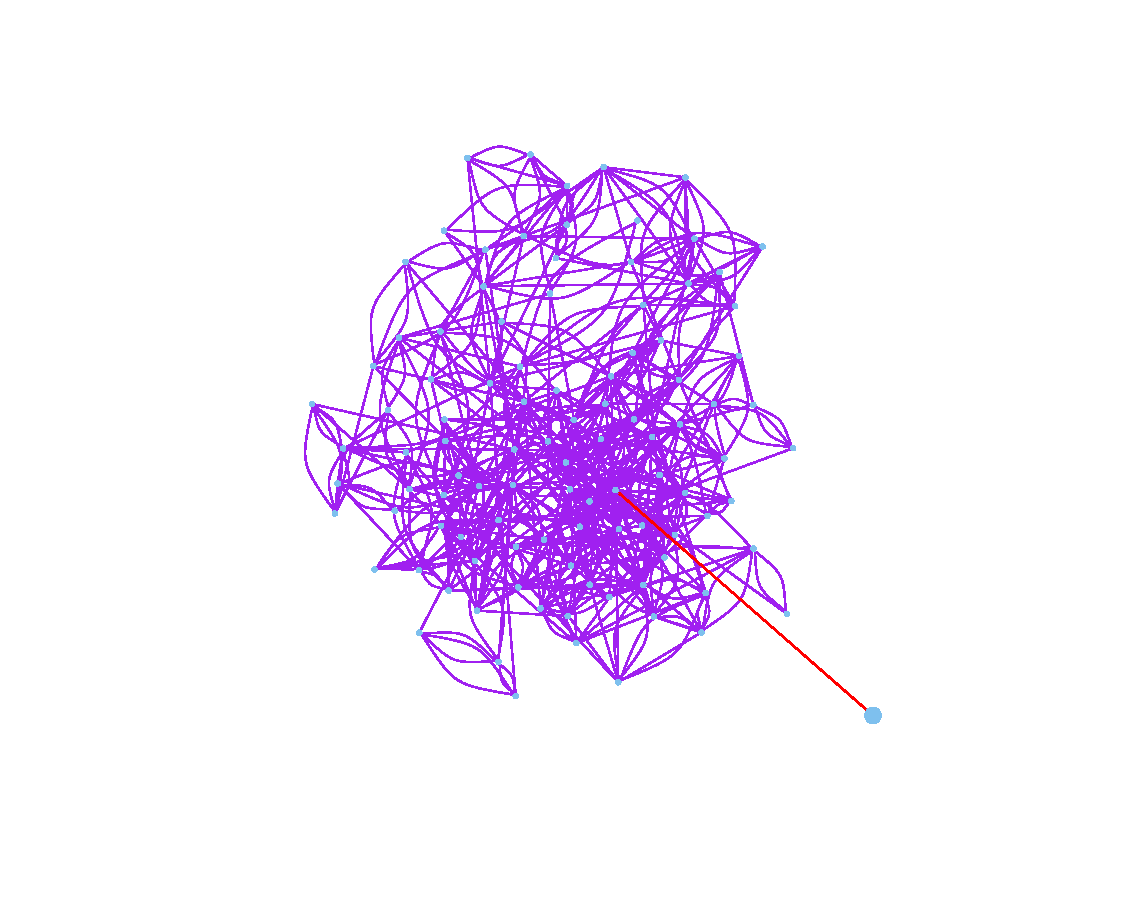
\includegraphics{manuscript-religion}
\caption{The same graph, showing the plot connections (red) and religious (purple) links.}
\end{rnwfig}

\begin{rnwfig}
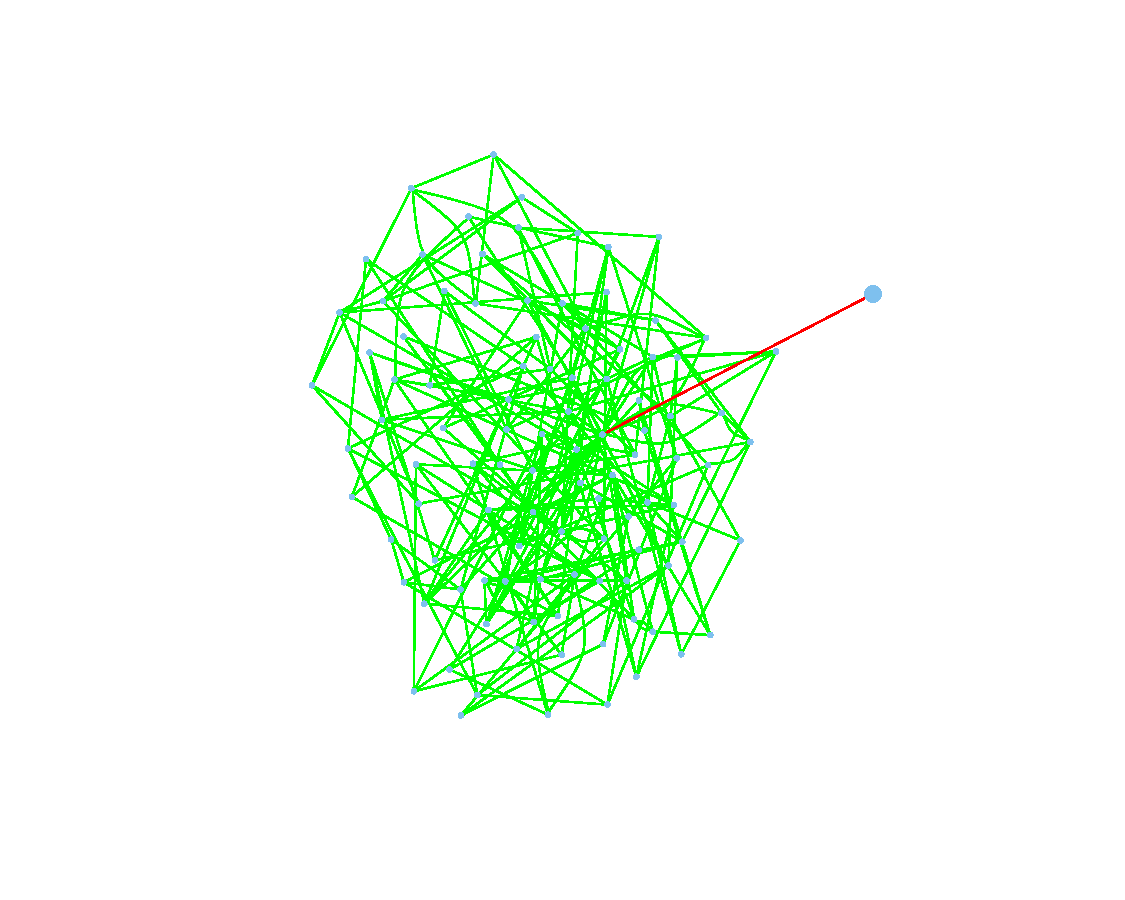
\includegraphics{manuscript-work}
\caption{Now showing work (green) links.}
\end{rnwfig}

\begin{rnwfig}
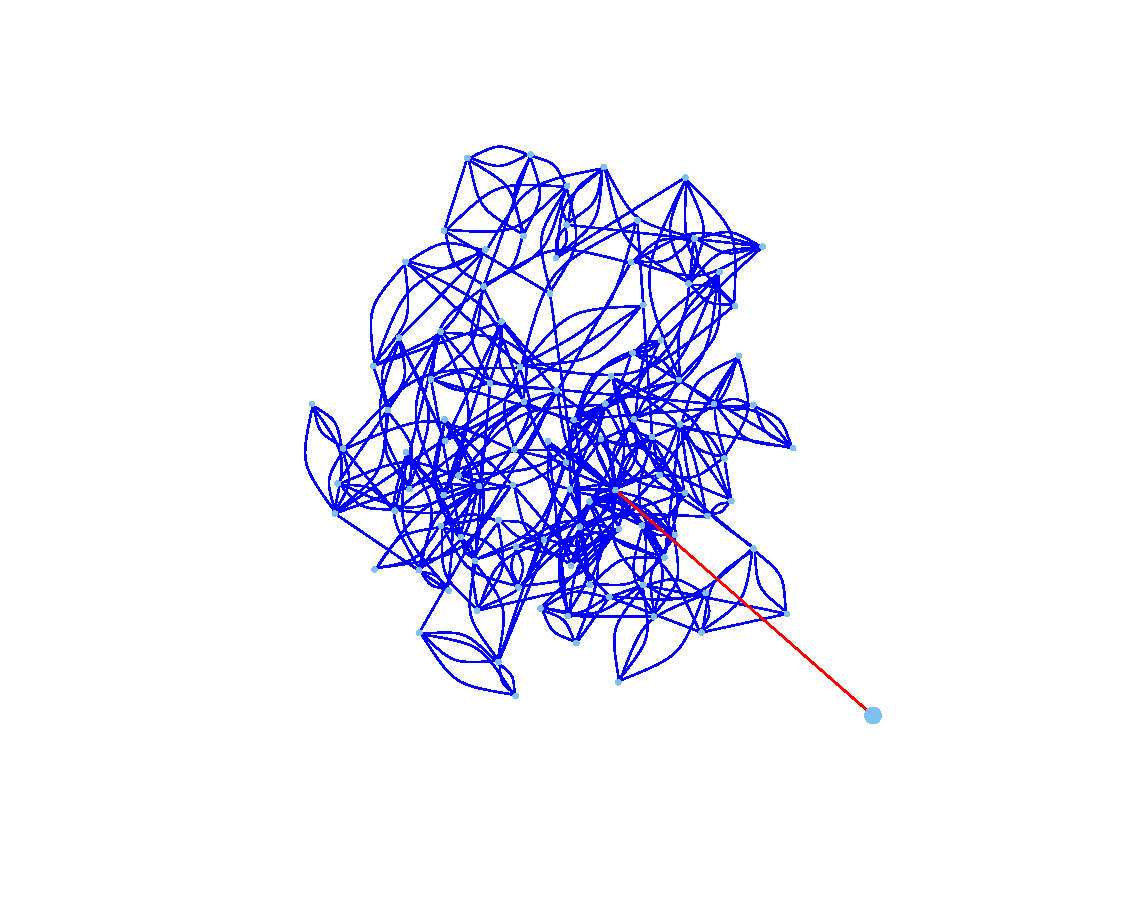
\includegraphics{manuscript-family}
\caption{Now showing family (blue) links.}
\end{rnwfig}

We also consider an alternative background: instead of cliques for ``Familial'' and ``Economic'' ties, individuals form trees.  The treatment for ``Religious'' ties remains the same.  The trees have a similar $n$ parameter for branching, and form bidirectional links.  This is obviously less sophisticated than the aforementioned hierarchical structures.  Is it less plausible as well?  Certainly, it seems off relative to, say, a NATO country: no interaction loops in a particular social context seems unimaginable.  Perhaps this is more reasonable in a setting where there is less information technology penetration or less observable interaction.  Perhaps its more plausible if the trees instead had siblings form cliques as well.  None of that supposition is particularly relevant: we picked another academic fiction to compare with our previous one.


\begin{rnwfig}
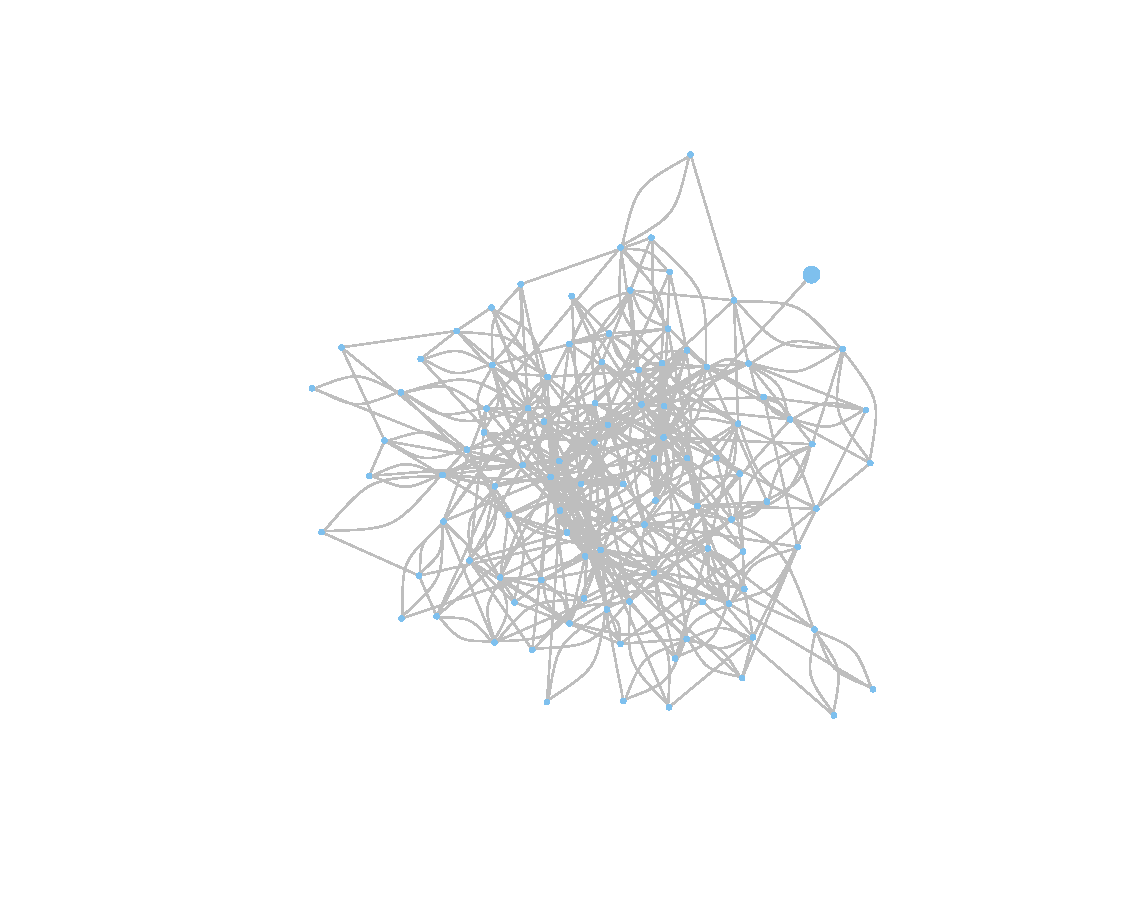
\includegraphics{manuscript-allAlt}
\caption{Overlay of all connections; again, the large vertex represents the cluster of subordinates.}
\end{rnwfig}

\begin{rnwfig}
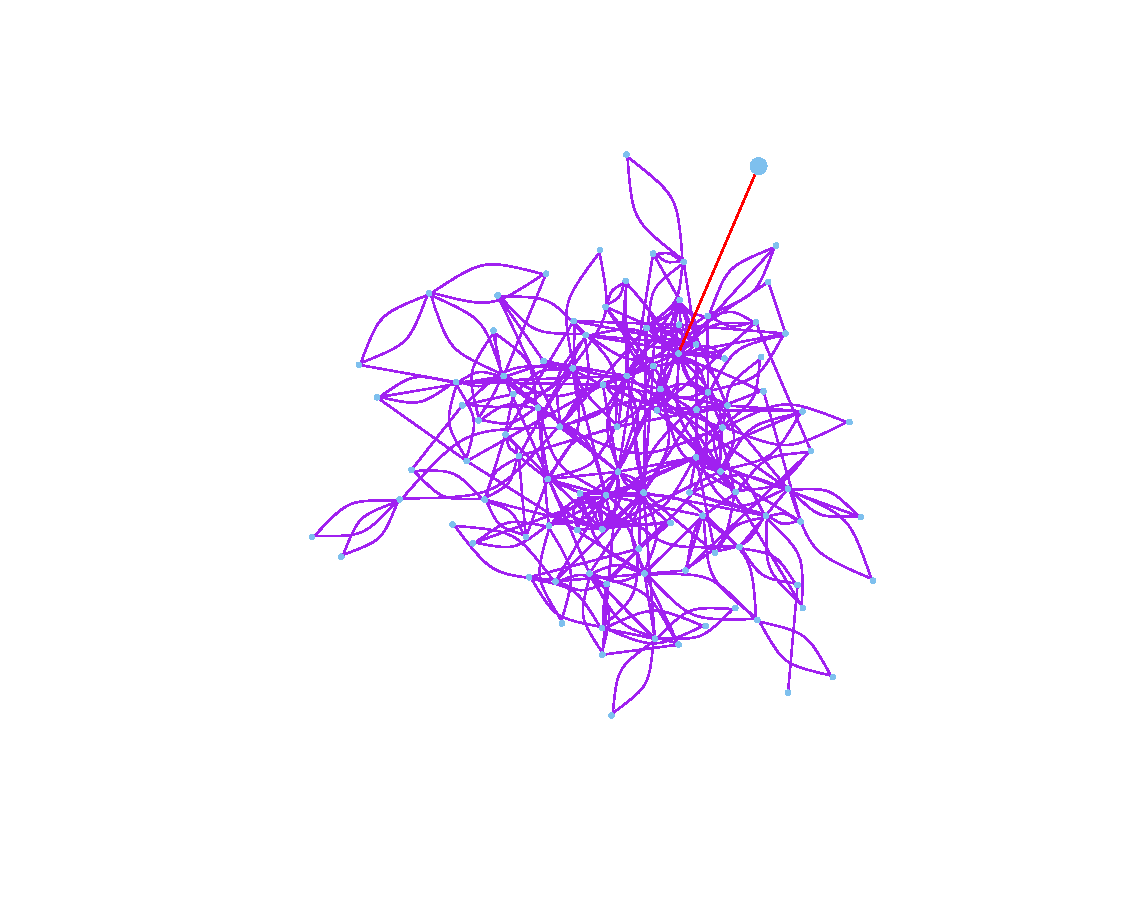
\includegraphics{manuscript-religionAlt}
\caption{The same graph, showing the plot connections (red) and religious (purple) links.}
\end{rnwfig}

\begin{rnwfig}
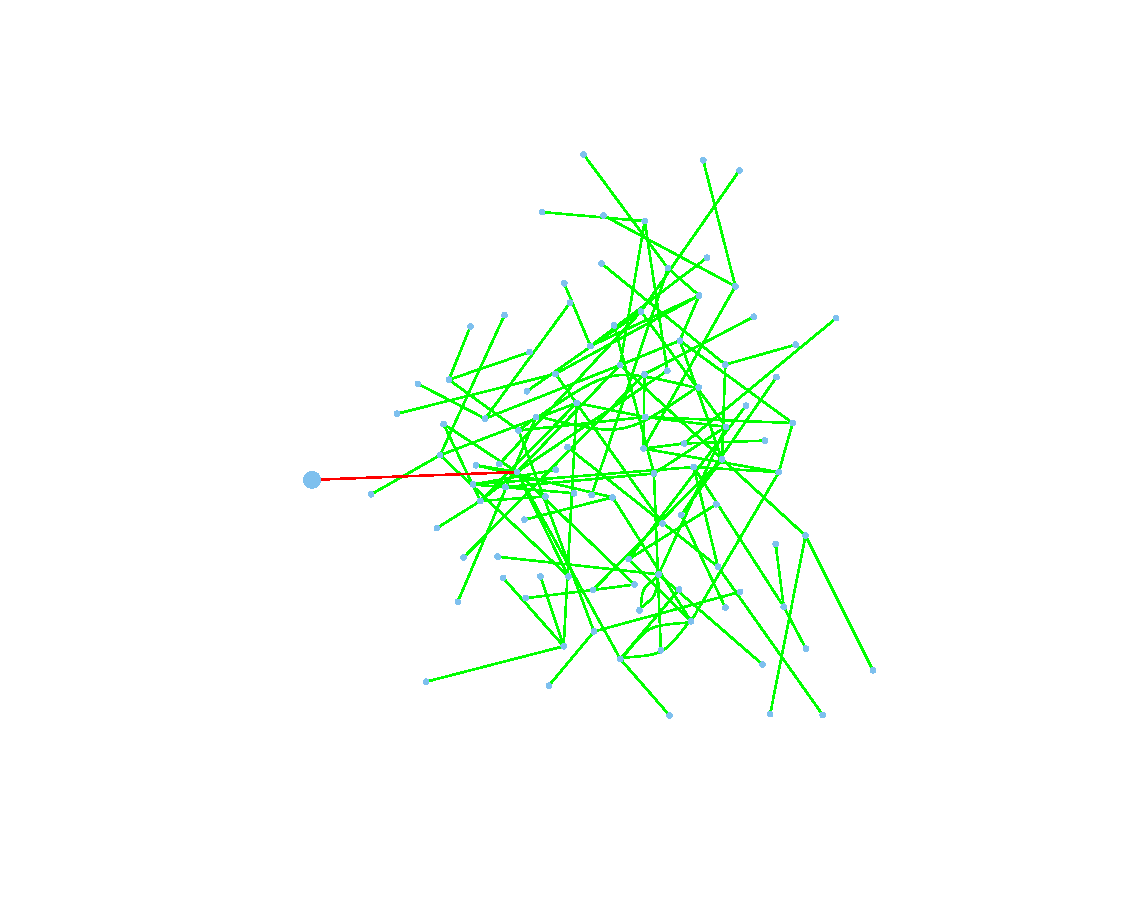
\includegraphics{manuscript-workAlt}
\caption{Now showing work (green) links.}
\end{rnwfig}

\begin{rnwfig}
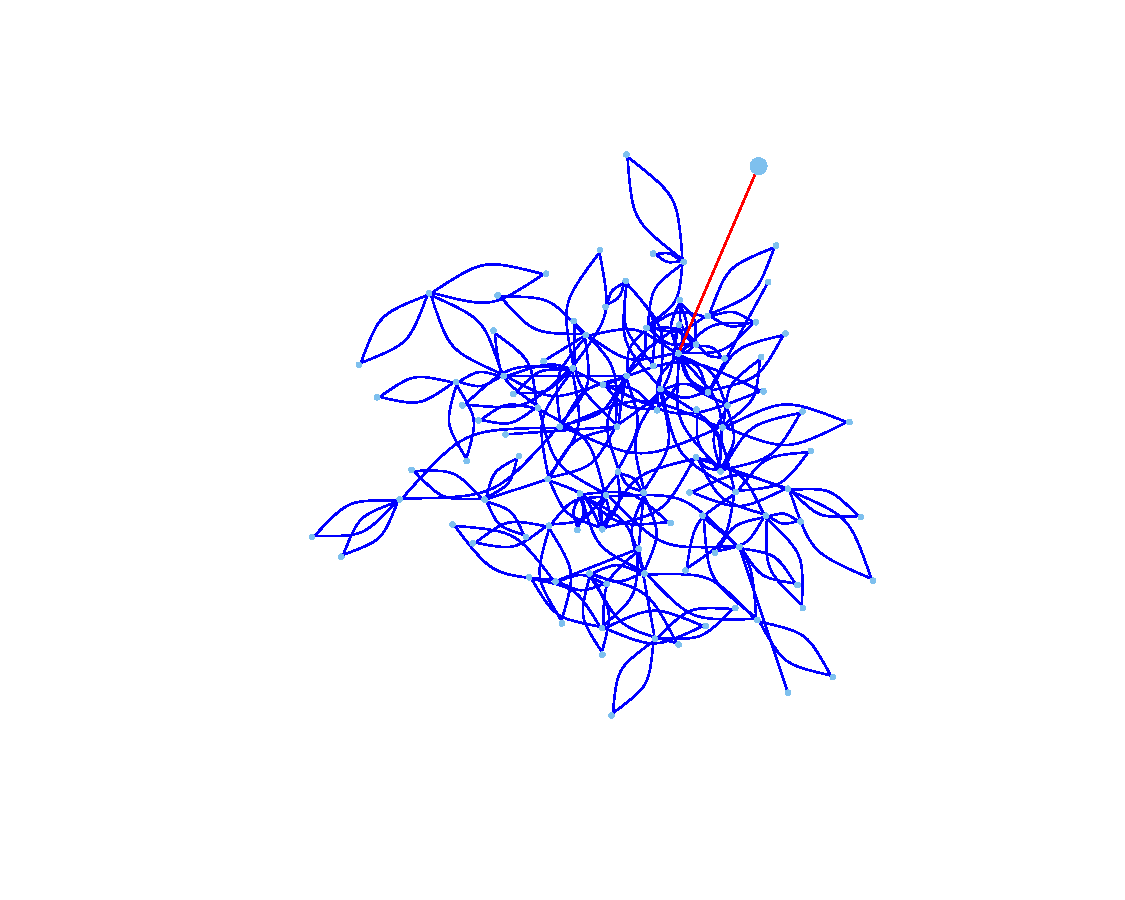
\includegraphics{manuscript-familyAlt}
\caption{Now showing family (blue) links.}
\end{rnwfig}

\subsubsection*{Covert Actors}
Sageman, Qin, et al. describe the structure of the Salafi networks as comprising a few key individuals with links to a large group of lieutenants -- the middle management of terror -- that are each connected to several tightly clustered subordinate groups -- terrorist cells -- that execute plots.  The lieutenants typically integrate with the regular population, while the subordinate groups are largely cloistered.

So we consider a covert organization consisting of two types, those directing a plot, {\em Management}, and those carrying out the day-to-day details, {\em Subordinates}.  For this demonstration model, we consider a ``small enough'' plot with a ``narrow enough'' schedule, such that only a single plot will occur during the simulation and that only a single manager is necessary to run that plot.

This manager, $M$, exists along side the background population.  Binomially sample the $C_i^0$ for ``Familial'' (with probability $p_F$) and ``Economic'' (with probability $p_E$) graphs and add $M$ to the selected $C_i^0$.  Then create ``Religious'' edges according to the same procedure used by ordinary individuals.

The subordinates, however, are isolated from the background population.  The manager and subordinates form a clique with a new type of edge: ``Plot''.

We also consider an alternative model: $M$ joins the background population as described above, but connects to the subordinate group via a hierarchical tree.

\subsection*{Modeling Action \&\ Observation}
Our proposed types have differences in their structural organization, but we also use those types to distinguish activity by those types on their related structure.  In this assessment, we represent activity only as monitorable communications, and those communications have their content flattened into two categories: ``Good'' and ``Bad''.  This is obviously a gross simplification of individual behavior (or over-estimation of analyst categorization capabilities); a potentially more appropriate version would be to have an abstract vocabulary with usage distinctions between the background and the clandestine group (e.g., uniform use in the background versus enriched in a subset in the clandestine group).  However, as we no doubt boringly emphasize: there is no particular basis for informing this model.  A time and group sensitive partitioning of intercepts for variety and distribution could plausibly form a basis for such a fit; one would have to consider, however, the distinction between the open source background communications (i.e., generally known to be public) versus the intercepted communications of the clandestine group (generally assumed private).

One last technical issue before proceeding to our example implementation: activity models may obviously differ in the data they generate, both structurally and semantically.  The underlying masking and investigating strategies may be framed relative to a particular action model, which may then require an adaptation of the activity data to be consistent with those adjacent models.

\subsubsection*{Background Action}
Each simulation time step, individuals in the background population generate messages by binomially sampling from all of their available connections.  They exhibit no preference for the type of those connections (beyond the structural consequence of having different numbers of different types).  If one interprets each message as a whole conversation, initiated by the sending party, then one implication of this model is that their messaging activity occupies an inconsequential period of real time relative to the real time equivalent of simulation step.  If one believed it was useful to model conversations explicitly -- i.e., each message is a word or phrase -- then one obvious change would be that individuals would only be selecting one target at a time, as well as modeling the speaker switch versus terminating communication.  This highlights a previously mentioned problem for the observation strategy -- there must exist an adapter for strategies between data types.  In this proposed continuous model, the aggregation for a strategy that only considers whole messages might be to average (on some specific real time scale) the total vocabulary in each direction of the conversation and then send one message from each party.

As for message content, the background population sends ``Good'' messages with a higher probability than ``Bad'' messages.

\subsubsection*{Covert Action}
The clandestine group's manager, $M$, behaves much like background population relative to his non-``Plot'' edges.  His tendency to send ``Bad'' messages to the background population is defined relative to the background probability.

However, he additionally sends direction to the subordinate group via the ``Plot'' connections with some probability.  Presumably, he would balance execution rate with secrecy.

The subordinates, however, do not interact with the background population.  They randomly speak with each other, with an enhanced probability of sending ``Bad'' messages after having received them from another member of the clandestine group.

\subsection*{Modeling Observation}
Incomplete information is the norm in these investigations, much like any work in the non-physical sciences.  However, it is typically possible to modulate what information is available (by investing more resources, by redirecting assets, etc).  We do not illustrate any strategies for either side in terms of modulating the flow of information, though an obvious addition dimension to add to both parties would be some resource pool that can be applied to modifying what information arrives at the observer (e.g., modulating the probability of detecting ``Bad'' messages from the covert group, faking messages in the background or to suspect members of the clandestine group).  For our simple model, we have different detection rates for the various edge flavors: ``Economic'' being highest, then ``Religious'', then ''Familial'', then ''Plot''.  The type of edge used to transmit the message is also not disclosed.

\subsection*{Modeling Reaction}
We rate investigating entities that implement a few different strategies.  One strategy is purely structural based on degrees, another purely content-oriented based on ``Bad'' frequency, and the third mixes the first two.

\subsubsection*{Structural Strategy}
Structural identification strategies range from having strong prior belief about a particular feature -- e.g., degree distribution -- and a relatively simple detection computation to belief only that there is a meaningful structural distinction (and a covert group to detect at all), thus running up against practical computational considerations trying to analyze all possible distinctions.

We demonstrate a case of the former, positing that the unique structural feature is to do with degree distribution -- specifically, a relatively high degree distribution for the manager, a relatively low degree distribution for the subordinates, and connection between them.  The criteria for labeling a member of the covert group is then a matter of setting what slices of the distribution to take from the top and bottom, and then testing for an observed path between the manager and the subordinate.

\subsubsection*{Content Strategy}
A pure content strategy ignores details about sender and receiver arrangement, instead focusing on the sending and receiving of different types of messages.  For our simple model, we consider a strategy that measures relative in and outflow of messages and the frequency of ``Bad'' messages.

\subsubsection*{Combination Strategy}
For our example combination strategy, we simply require individuals pass both threshold measures.

\section*{Evaluation}
There are two basic aspects of evaluation, which correspond to the general scientific method questions of model fitting versus model selection.  Note that these are entirely separate from detailed application of these aspects to particular model components; those activities are certainly critical in narrow assessments, but we must again emphasize the ability of both sides to adapt their strategies, improve technological capabilities, and so on, all of which will present disruptive changes to any established model.

The aspect which corresponds to questions of fit is basically identifying, for a particular model context -- specific combination of opposed strategies and background activity -- parameter surfaces for optimal performance on the chosen metrics.

The question of model selection corresponds more to considering these performance surfaces across a wide breadth of combinations.  That is, how well does a particular covert strategy perform across multiple background population behaviors and against varying investigatory capabilities?  Vice versa for the investigatory system?

For our toy systems we consider a simple performance metric, the Receiver Operator Characteristic discrimination statistic, across a background parameter sweep and as a function of time duration. 

\subsection*{Structural Performance}
\begin{rnwfig}
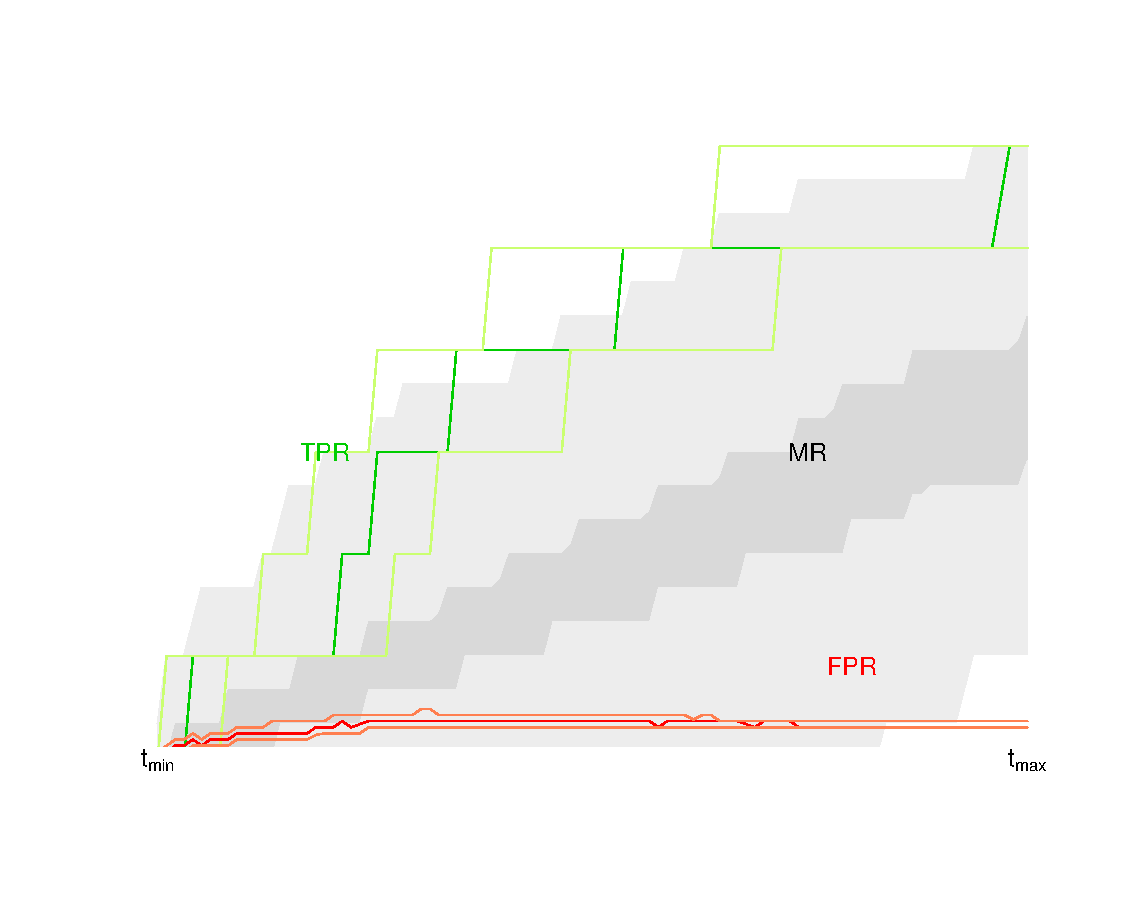
\includegraphics{manuscript-structure}
\caption{Structure-Only performance versus clique-based background.}
\end{rnwfig}

\begin{rnwfig}
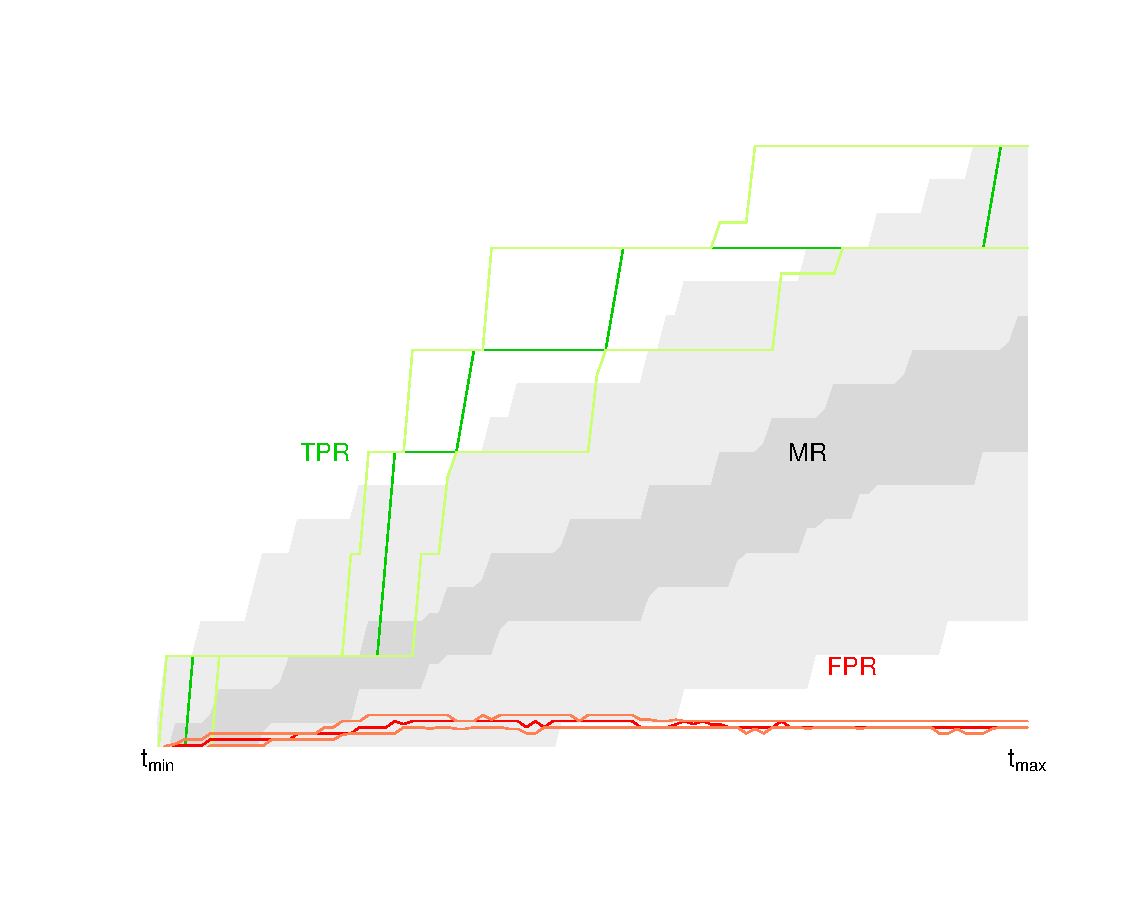
\includegraphics{manuscript-astructure}
\caption{Structure-Only performance versus tree-based background.}
\end{rnwfig}

\begin{rnwfig}
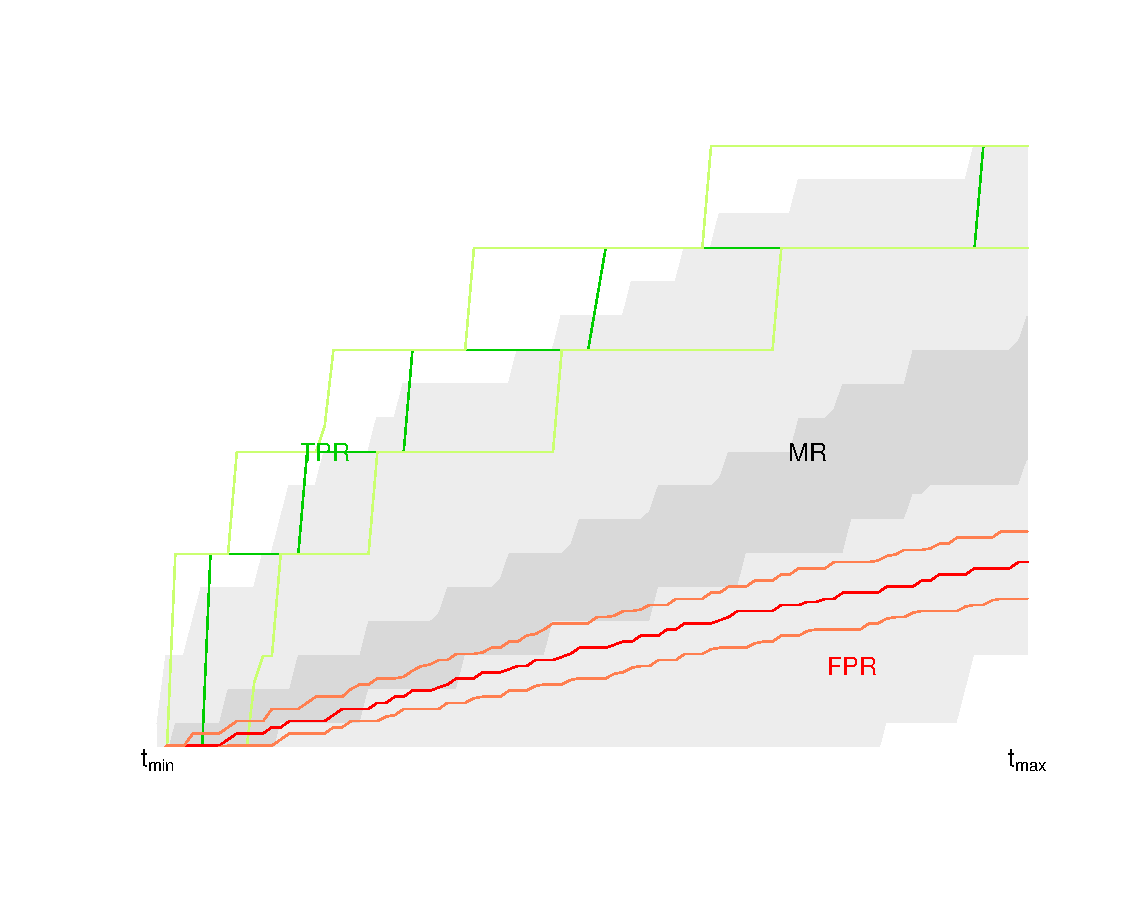
\includegraphics{manuscript-content}
\caption{Content-Only performance versus clique-based background.}
\end{rnwfig}

\begin{rnwfig}
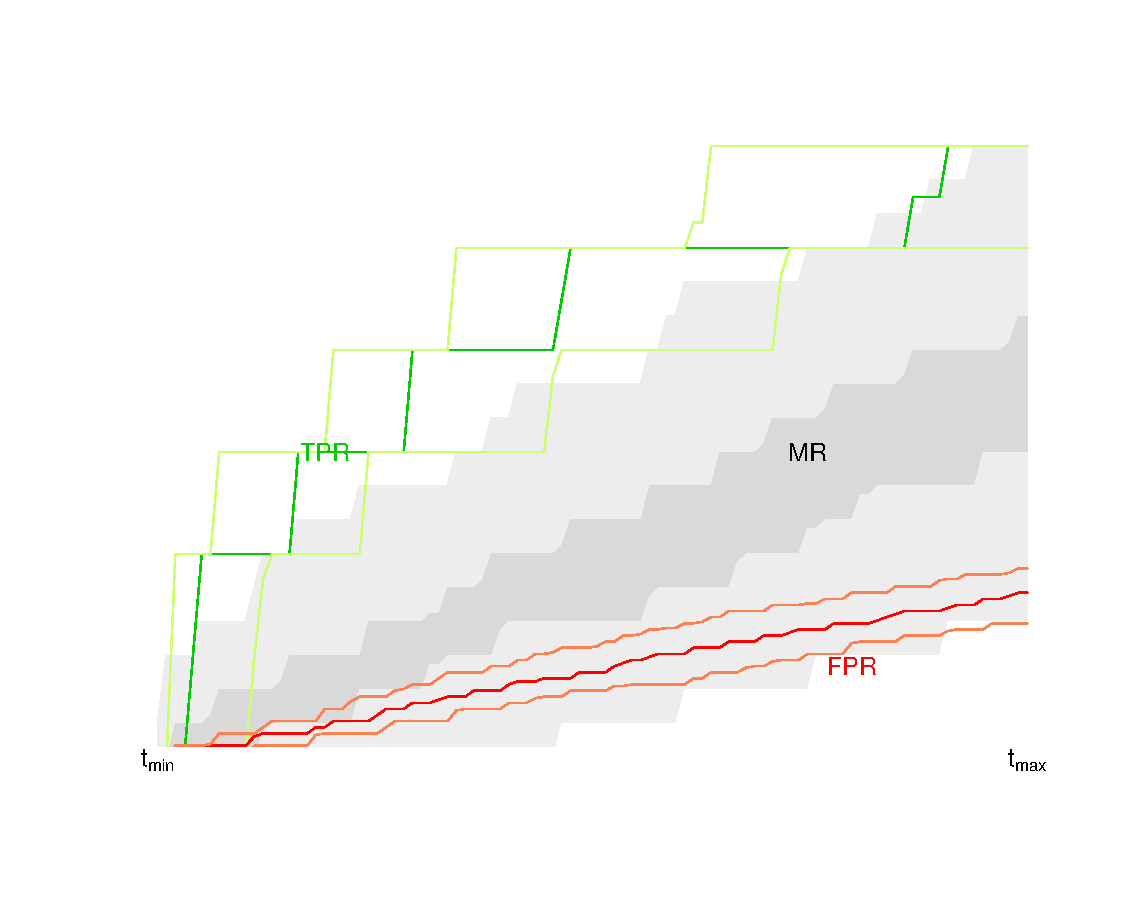
\includegraphics{manuscript-acontent}
\caption{Content-Only performance versus tree-based background.}
\end{rnwfig}

\begin{rnwfig}
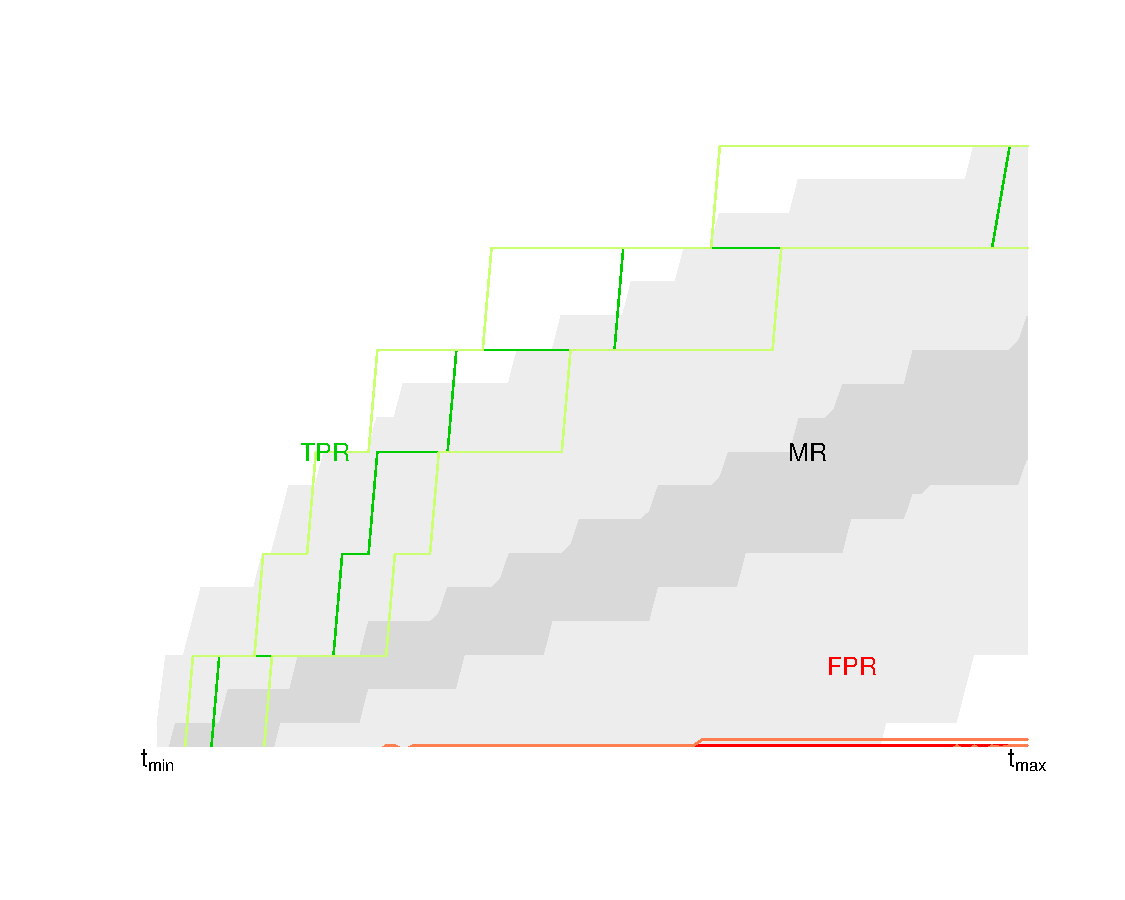
\includegraphics{manuscript-sandcontent}
\caption{Structure and Content performance versus clique-based background.}
\end{rnwfig}

\begin{rnwfig}
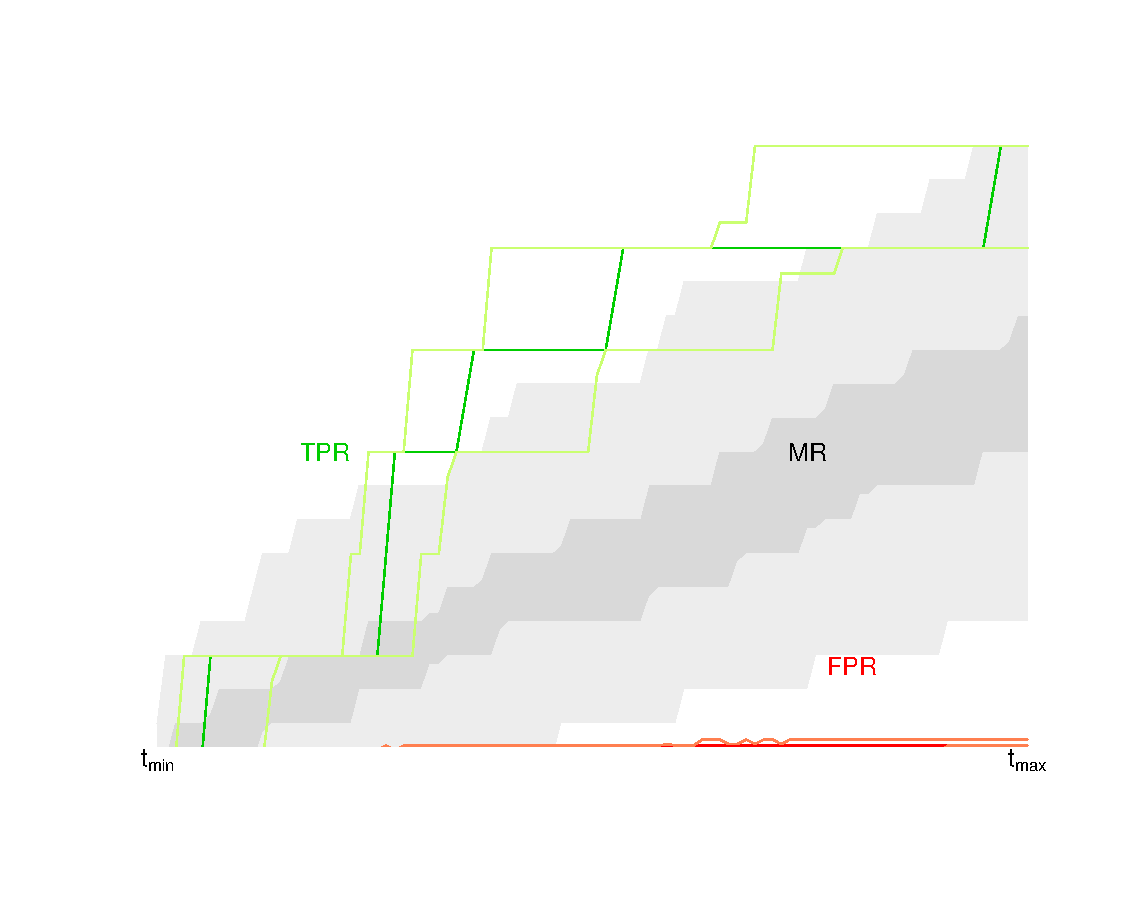
\includegraphics{manuscript-asandcontent}
\caption{Structure and Content performance versus clique-based background.}
\end{rnwfig}

\section*{Discussion}
\todoCP{Get figures to give some direction for this.  Probably going to see the interesting stuff in the differently organized pops.}

\end{document}
